% Sample file on how to use subfiles.
\documentclass[ExampleMasters.tex]{subfiles}

\begin{document}
\clearpage
\chapter{Vehicle Model controllers (3 Seiten)}
\label{chap:steering_model}
There are two different controllers used to control the steerable axles of the dolly. One is used for low-speed and one for high-speed maneuvers. The main purpose of the low-speed controller is the reduction of off-tracking.
For the high-speed controller the aim is to reduce the rearward amplification.
\section{Low-Speed controller \cite{Low-speed_paper}}
\label{sec:low-speed_controller}
The low-speed controller is implemented in path-distance domain $\eta$. The path-distance is calculated by integrating the forward speed $v_{x,1}(t)$. \\
The steering angle of the first axle of the dolly is calculated as follows: 
\begin{equation}
\delta_{31}(\eta)=k_1\delta_{11}(\eta-\eta_1)+k_2\Delta\psi_1(\eta-\eta_2)+k_3\Delta\psi_2(\eta-\eta_3)+k_4\Delta\psi_3(\eta-\eta_4)
\end{equation}
\label{eq:delta31_lowspeed}
where $\delta_{31}$ is the steering angle of the dolly's front axle, $\delta_{11}$ is the steering angle of the tractor's front axle, $\Delta\psi_1$ the articulation angle between the tractor and the first semitrailer, $\Delta\psi_2$ the articulation angle between the first semitrailer and the dolly, $\Delta\psi_3$ the articulation angle between the dolly and the second semitrailer, $\eta_1$ the distance between the tractor's first axle and the dolly's first axle, $\eta_2$ the distance between the first articulation joint and the dolly's first axle, $\eta_3$ the distance between the second articulation joint and the dolly's first axle, $\eta_4$ the distance between the third articulation joint and the dolly's first axle, and $k_1, k_2, k_3, k_4$ are gains. 
\\The steering angle of the second axle of the dolly is calculated using the steering angle of the first dolly axle as follows:
\begin{equation}
\delta_{32}(\eta)=k_5\delta_{31}(\eta-\eta_5)
\end{equation}
\label{eq:delta32_lowspeed}
where $\delta_{32}$ is the steering angle of the dolly's second axle, $\eta_5$ is the distance between the dolly's second and first axle, and $k_5$ is a gain.\\
The gains $k_1, k_2, k_3, k_4, k_5$ were optimized using the particle swarm optimization.
Table \ref{tab:gains_after_optimization} shows the values of the gains after the optimization and the improvement of the controller for different maneuvers.
\begin{table}[h]
	\centering
	\caption{Control gains and performance improvement}
	\label{tab:gains_after_optimization}
	\begin{tabular}{l|l|l l l}
		& &  & Improvement  \\ \hline
		Gain & Value & 180-deg turn (\%) & 90-deg turn (\%) & S-turn\\ \hline
		$k_1$   &       -0.2126      &             \\
		$k_2$    &            -0.1567 &             \\
		$k_3$  &      -0.8780       &           +44.61 & +37.75 & +45.07  \\
		$k_4$ &      -0.3143       &           \\
		$k_5$  & 0.9868 & \\
		
	\end{tabular} \\
\end{table}\\
Figure \ref{fig:low_speed_diagram} shows the implementation of the controller in the functional architecture.

\begin{figure}[h]
	\centering
	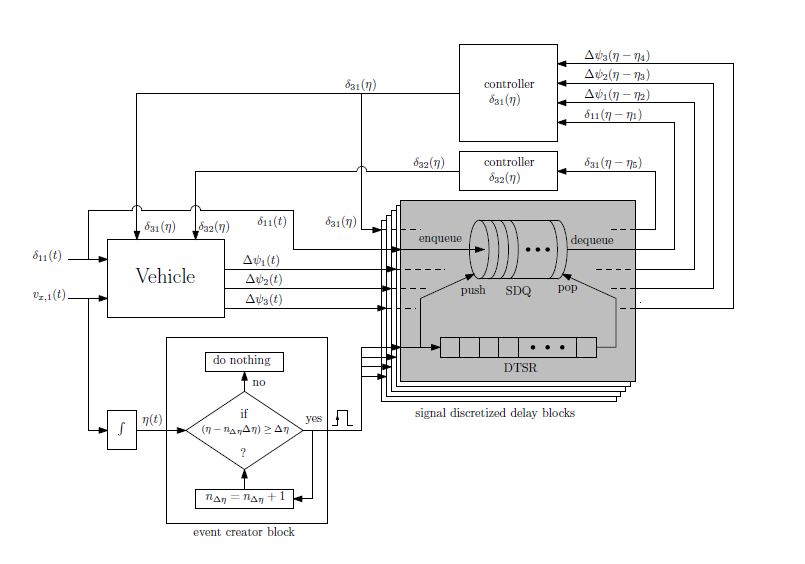
\includegraphics[width=1.0\linewidth]{figures/Low_speed_diagram}
	\caption[]{Controller implementation in the functional architecture \cite{Low-speed_paper}}
	\label{fig:low_speed_diagram}
\end{figure}

\subsection{Input parameters}
\label{sec:input_parameters_LS}
The input parameters for the low-speed controller are:
\begin{itemize}
	\item The articulation angles between the different units: $\Delta\psi_1$, $\Delta\psi_2$, $\Delta\psi_3$
	\item The steering angle of the tractor's first axle: $\delta_{11}$
	\item The distances of the tractor's first axle, the articulation joints of the different units and the dolly's second axle to the dolly's first axle: $\eta_1,\eta_2,\eta_3,\eta_4,\eta_5$
	\item The vehicle speed for the transformation from time to path-distance domain:  $v_x$
	
\end{itemize}

\section{High-Speed controller}
\label{sec:high-speed_controller}
The high-speed controller is implemented using a nonlinear inverse of a dynamic vehicle model.
\begin{itemize}

\item same path of all units --> time delay of units considered
\item lateral acceleration of dolly(t) = lat. accel. of truck(t-tau)
\item modelica used because it can do inverse models
\item imported to simulink as a functional mock-up unit (FMU) using FMI-toolbox
\subsection{Input parameters}
\label{sec:input_parameters_HS}

\begin{itemize}
	\item ay3ref = delayed ay1
	\item ay3; delta11, vx
	\item derivative of delta11 needed for inversion operation
	\item explain feedback/inverse path
	
\end{itemize}

\end{itemize}
 \begin{figure}[h]
 	\centering
 	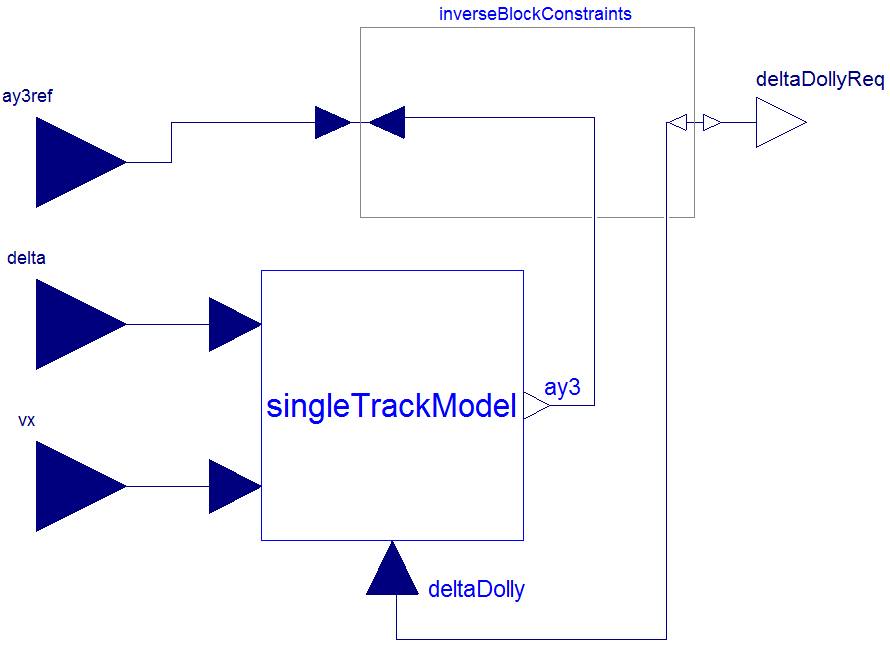
\includegraphics[width=1.0\linewidth]{figures/Inverse_of_A-double_single-track}
 	\caption[]{Inverse of the single track A-double model \cite{High-speed_paper}}
 
 	\label{fig:inverse_model}
 \end{figure}
 
\section{Overview of the model}
\label{sec:overview_of_the_model}
			
\begin{itemize}
	\item based on lit from MI-paper 
	\item overview graph of model
	\item single track model
	
	\item filtering of inputs?
	\item feedback-loop
	\item start condition
	\item what can be concluded with the model?
\end{itemize}



\section{Real-Time implementation of controllers}
\label{sec:real_time_implementation}

\begin{itemize}
	\item this paragraph in close cooperation with MI
	\item what had to be changed to allow for MABII execution?
	\item how will feedback loop be handled?
	item incorporate measurings?
	\item simulation step size?
	\item utilized computational method
\end{itemize}

\section{Interface with Real-Time environment}
\label{sec:interface_with_real_time}

\begin{itemize}
	\item capabilities of system (see section \ref{sec:maxi_capabilities})
	\item signals passed forward from environment + restriction
	
	\item actuator signals
	\item signal modification (correct frequency for CAN)
	\item safety flags/signals
	
\end{itemize}

\end{document}
